
\section{Results}\label{sec:results}
Figures~\ref{fig:_mu12},~\ref{fig:pTb1}, and~\ref{fig:pTmu1} show relevant kinematic distributions for two benchmark signal points and the dominant SM backgrounds, using the subset of events passing the pre-selections defined above. The signal benchmark points in these figures are $m(\phi^{'}) = 325 \, \mathrm{GeV}$, $m(\chi_{\mathrm{u}}) = 2\, \mathrm{TeV}$, and $m(\phi^{'}) = 1 \, \mathrm{GeV}$, $m(\chi_{\mathrm{u}}) = 500\, \mathrm{GeV}$. The distributions are normalized such that the area under the curve is unity. These distributions correspond to the reconstructed mass, $m(\mu_{1}, \mu_{2})$, between the two muon candidates with the highest transverse momentum ($\mu_{1}$ and $\mu_{2}$), 
the transverse momentum of the b-jet candidate with the highest transverse momentum $p_{\mathrm{T}}$ ($\mathrm{b_{1}}$), and the muon candidate with the highest transverse momentum $p_{\mathrm{T}}$ ($\mu_{1}$), respectively. 
These distributions are among the variables identified by the BDT algorithm with the highest signal to background discrimination power (see Figure~\ref{fig:feature_importance}).

As can be seen from Figure~\ref{fig:_mu12}, the $\phi'$ mass can be reconstructed through its associated muon decay pair, which is observed as a peak in the $m(\mu_{1}, \mu_{2})$ distribution around the expected $m(\phi')$ value, and has low- and high-mass tails which are a consequence of cases where the leading and/or subleading muon is not from the $\phi'$ decay, but rather from the associated $\mathrm{W}$ boson from the $\chi_{\mathrm{u}}$ decay. For the backgrounds, muons come from \textrm{Z} (\textrm{W}) decays. Therefore, the $m(\mu_{1}, \mu_{2})$ background distributions show a peak near $m_{\mathrm{W/Z}}$, combined with a broad distribution indicative of the combination of two muon candidates from different decay vertices. We note that the $\phi'\to\mu^{+}\mu^{-}$ decay width depends on the square of the $\phi'\to\mu^{+}\mu^{-}$ coupling and  $\frac{m_{\mu}^{2}}{m(\phi')^{2}}$ and is thus suppressed by the relatively small muon mass. For the new physics phase space considered in this paper, the $\phi'$ decay width is less than 1\% of the $\phi'$ resonant mass. Furthermore, as indicated previously, the signal/background interference effects are small and negligible compared to effects from experimental resolution. Therefore, the width of the $m(\mu_{1}, \mu_{2})$ signal distributions is driven by the experimental resolution in the reconstruction of the muon momenta, as well as the probability that the two leading muons are the correct pair from the $\phi'$ decay. Since the probability that the two highest-$p_{\mathrm{T}}$ muons are the correct pair from the $\phi'\to\mu^{+}\mu^{-}$ decay depends on $m(\phi')$ and $m(\chi_\mathrm{u})$, it is important to include all possible combinations of dimuon pairs (i.e., $m(\mu_{1}, \mu_{3})$ and $m(\mu_{2}, \mu_{3})$) in the training of the BDT. 

Figure~\ref{fig:pTb1} shows the  distribution for the \textrm{b}-jet candidate with the highest $p_{\mathrm{T}}$, $p_{\mathrm{T}}(\mathrm{b}_1)$, for the same simulated samples shown in Figure~\ref{fig:_mu12}. Based on the signal topology and our choice of parameter space (i.e., $m(\chi_\mathrm{u}) > m_{\mathrm{t}}$), it is expected that the leading $\mathrm{b}$-jet candidate comes from the $\chi_\mathrm{u}$ decay, with an average $p_{\mathrm{T}}$ close to $\frac{m(\chi_\mathrm{u}) - m_{\mathrm{W}}}{2}$, as observed in Figure~\ref{fig:pTb1}. For the $\mathrm{t} \overline{\mathrm{t}} \mu^{+}\mu^{-}$ background, the \textrm{b}-jet candidates come from top-quark decays. Therefore, their average transverse momentum is expected to be $\frac{m_{\mathrm{t}} - m_{\mathrm{W}}}{2} \approx 45$~\textrm{GeV}, as observed in Figure~\ref{fig:pTb1}. On the other hand, the \textrm{b}-jet candidates for the $\mathrm{b} \overline{\mathrm{b}}\mu\mu\mu\nu$ background can come from off-mass-shell $\mathrm{Z}^{*}/\gamma^{*}$, and thus typically have an even softer spectrum in comparison to the $\mathrm{t} \overline{\mathrm{t}} \mu^{+}\mu^{-}$ background.

Figure~\ref{fig:pTmu1} shows the  distribution for the muon candidate with the highest $p_{\mathrm{T}}$, $p_{\mathrm{T}}(\mu_{1})$. Similar to Figure~\ref{fig:pTb1}, when $m(\chi_\mathrm{u}) > m_{\mathrm{t}}$ it is expected that the leading muon candidate comes from the $\chi_\mathrm{u}$ decay, with an average $p_{\mathrm{T}}$ of approximately $\frac{m(\chi_\mathrm{u}) - m_{\mathrm{W}}}{4}$, as observed in Figure~\ref{fig:pTmu1}. For the major SM backgrounds, the muon candidates come from Z/W/$\gamma^{*}$ decays. Therefore, their average transverse momentum is expected to be much lower, $\frac{m_{\mathrm{Z/W}}}{4} \approx 40-45$~\textrm{GeV}. This kinematic feature provides a nice handle to discriminate high $m(\chi_\mathrm{u})$ signal events amongst the large SM backgrounds, which have lower average $p_{\textrm{T}}(\mu)$ constrained by the SM weak boson masses.

In addition to these aforementioned variables in Figures~\ref{fig:_mu12}-\ref{fig:pTmu1}, several other kinematic variables were included as inputs to the BDT algorithm. In particular, 27 such variables were used in total, and these included the momenta of $\mathrm{b}$ and muon candidates; invariant masses of pairs of muons; angular differences between $\mathrm{b}$ jets and between the muons. 

As mentioned above, the variables $m(\mu_{i}, \mu_{j})$ for $i, j \neq 1$ provide some additional discrimination between signal and background when the leading muons are not a $\phi'$ decay candidate. The angular separation variables, such as $\Delta R(\mu_{i}, \mu_{j})$, are designed to be sensitive to lower mass $\phi'$, since the low rest mass of those particles means they acquire more boost, and thus smaller angular separation $\Delta R$ between the muon candidates. The trained BDT returns the discriminating power of each of its inputs, and the feature importance for each variable is shown in Figure~\ref{fig:feature_importance} for a signal benchmark point with $m(\phi')=325\, \mathrm{GeV}$ and $m(\chi_\mathrm{u})=2000\, \mathrm{GeV}$.

\begin{figure}
\centering
  \centering  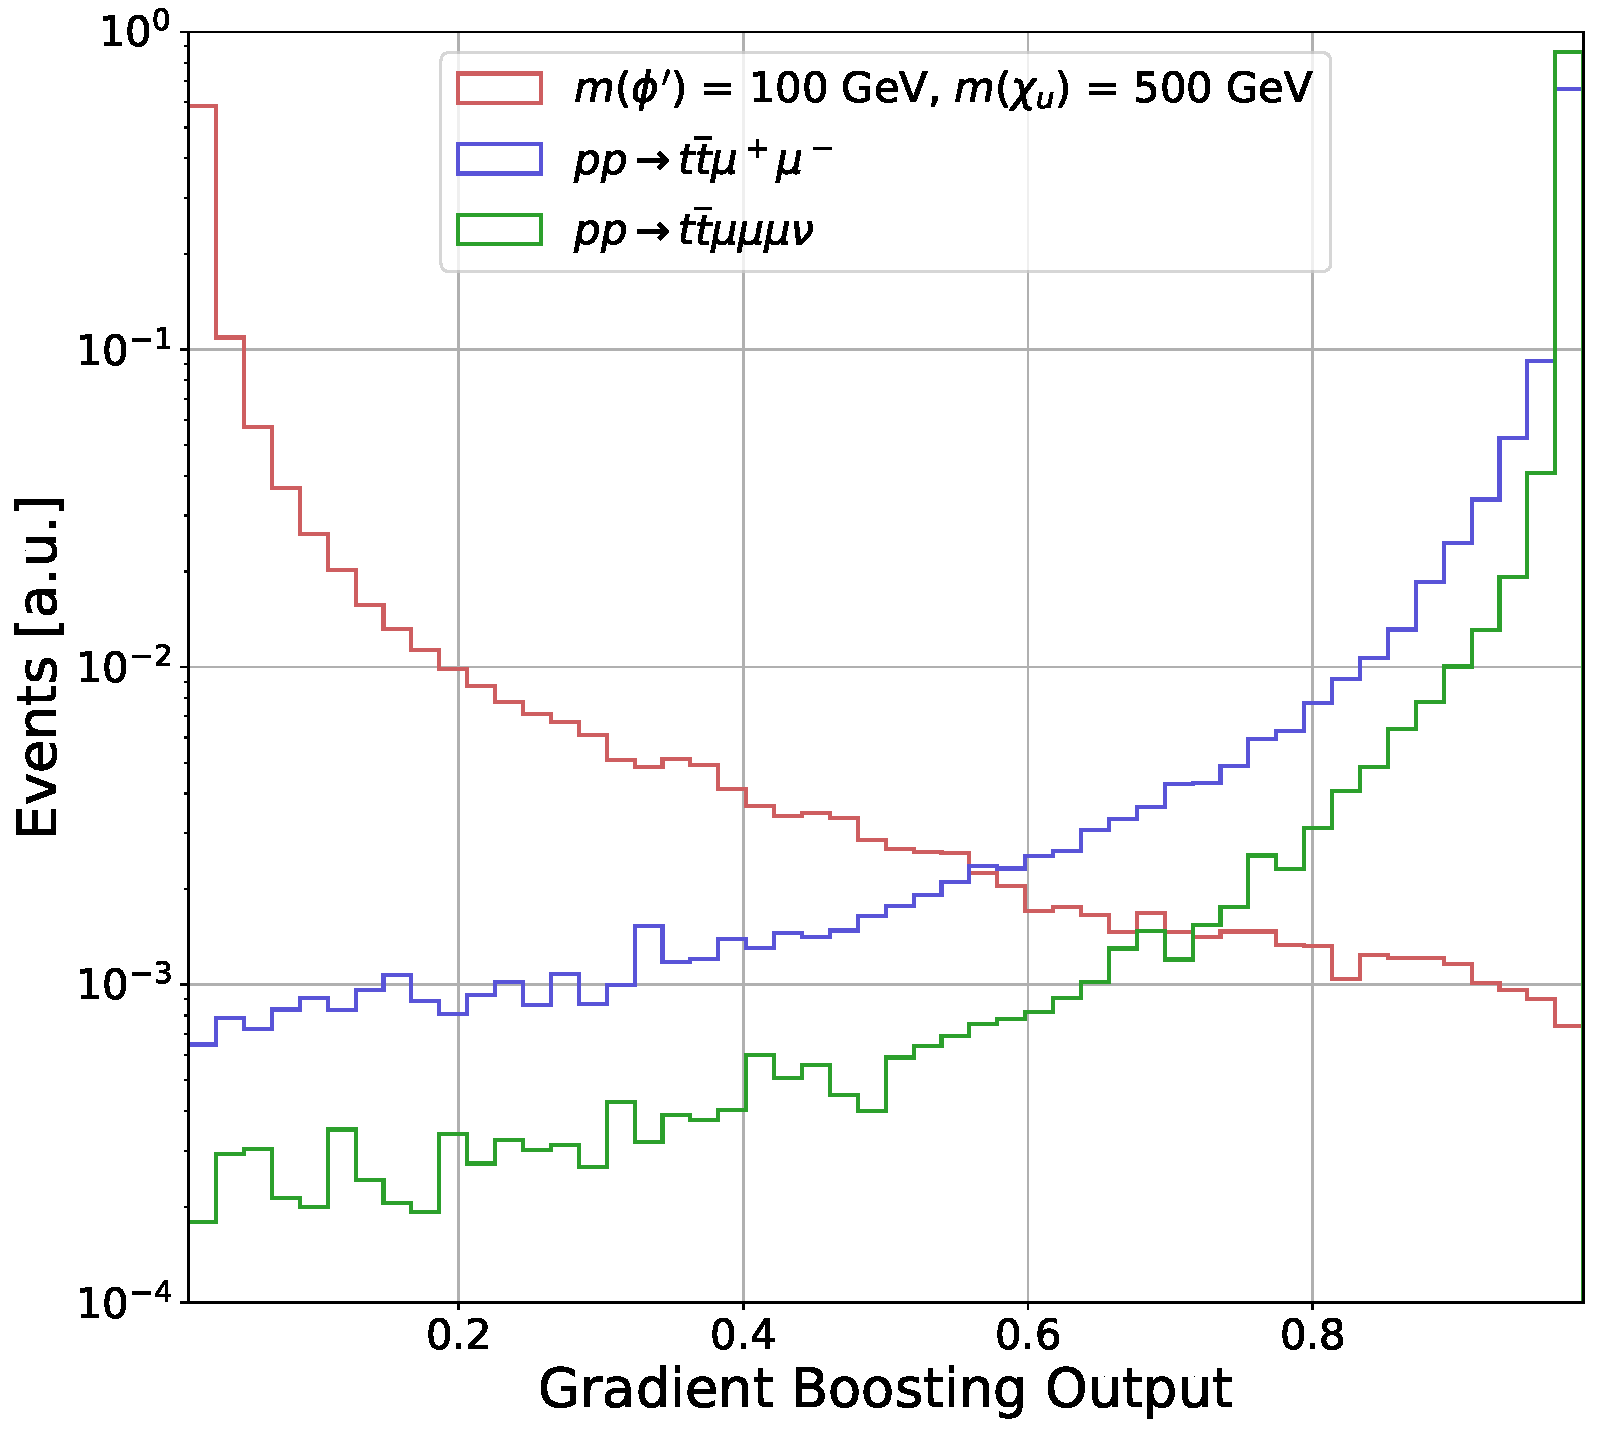
\includegraphics[width=.75\linewidth]{Images/XGB_output.pdf}
  \caption{Output of the gradient boosting algorithm for a benchmark $m(\phi') = 100$~\textrm{GeV} and $m(\chi_\mathrm{u}) = 500\, \mathrm{GeV}$ signal, and dominant backgrounds. The distributions are normalized to unity.}
  \label{fig:xgboostout}
\end{figure}

Figure~\ref{fig:xgboostout} shows  the distributions for the output of the BDT algorithm, normalized to unity, for the representative signal benchmark point of $m(\phi') = 1\, \mathrm{GeV}$, $m(\chi_\mathrm{u}) = 0.5\, \mathrm{TeV}$ and the two dominant backgrounds. The output of the BDT algorithm is a value between 0 and 1, which quantifies the likelihood that an event is either background-like (BDT output near 1) or signal-like (BDT output near 0). Figure~\ref{fig:ROC} illustrates the true positive rate (TPR), defined as the probability of correctly selecting signal events using the BDT output, plotted against the false positive rate (FPR), defined as the probability of incorrectly selecting background events. For example, for $m(\phi') = 100\, \mathrm{GeV}$ and $m(\chi_\mathrm{u}) = 500\, \mathrm{GeV}$, when signal events are selected at 65\% probability, the background is selected at about $10^{-3}$ probability. We note that the primary discriminating feature between the signal and background is the boosted b-jet $p_T$ coming from the $\chi_u$ vector-like quark. The $p_T$ of said b jet increases with $m(\chi_\mathrm{u})$, peaking at around $[m(\chi_\mathrm{u}) - m(\textrm{W})] / 2$. This enhanced boost increases the separation between signal and background, improving the performance of the BDT algorithm as $m(\chi_\mathrm{u})$ increases. 

\begin{figure}
\centering
  \centering
  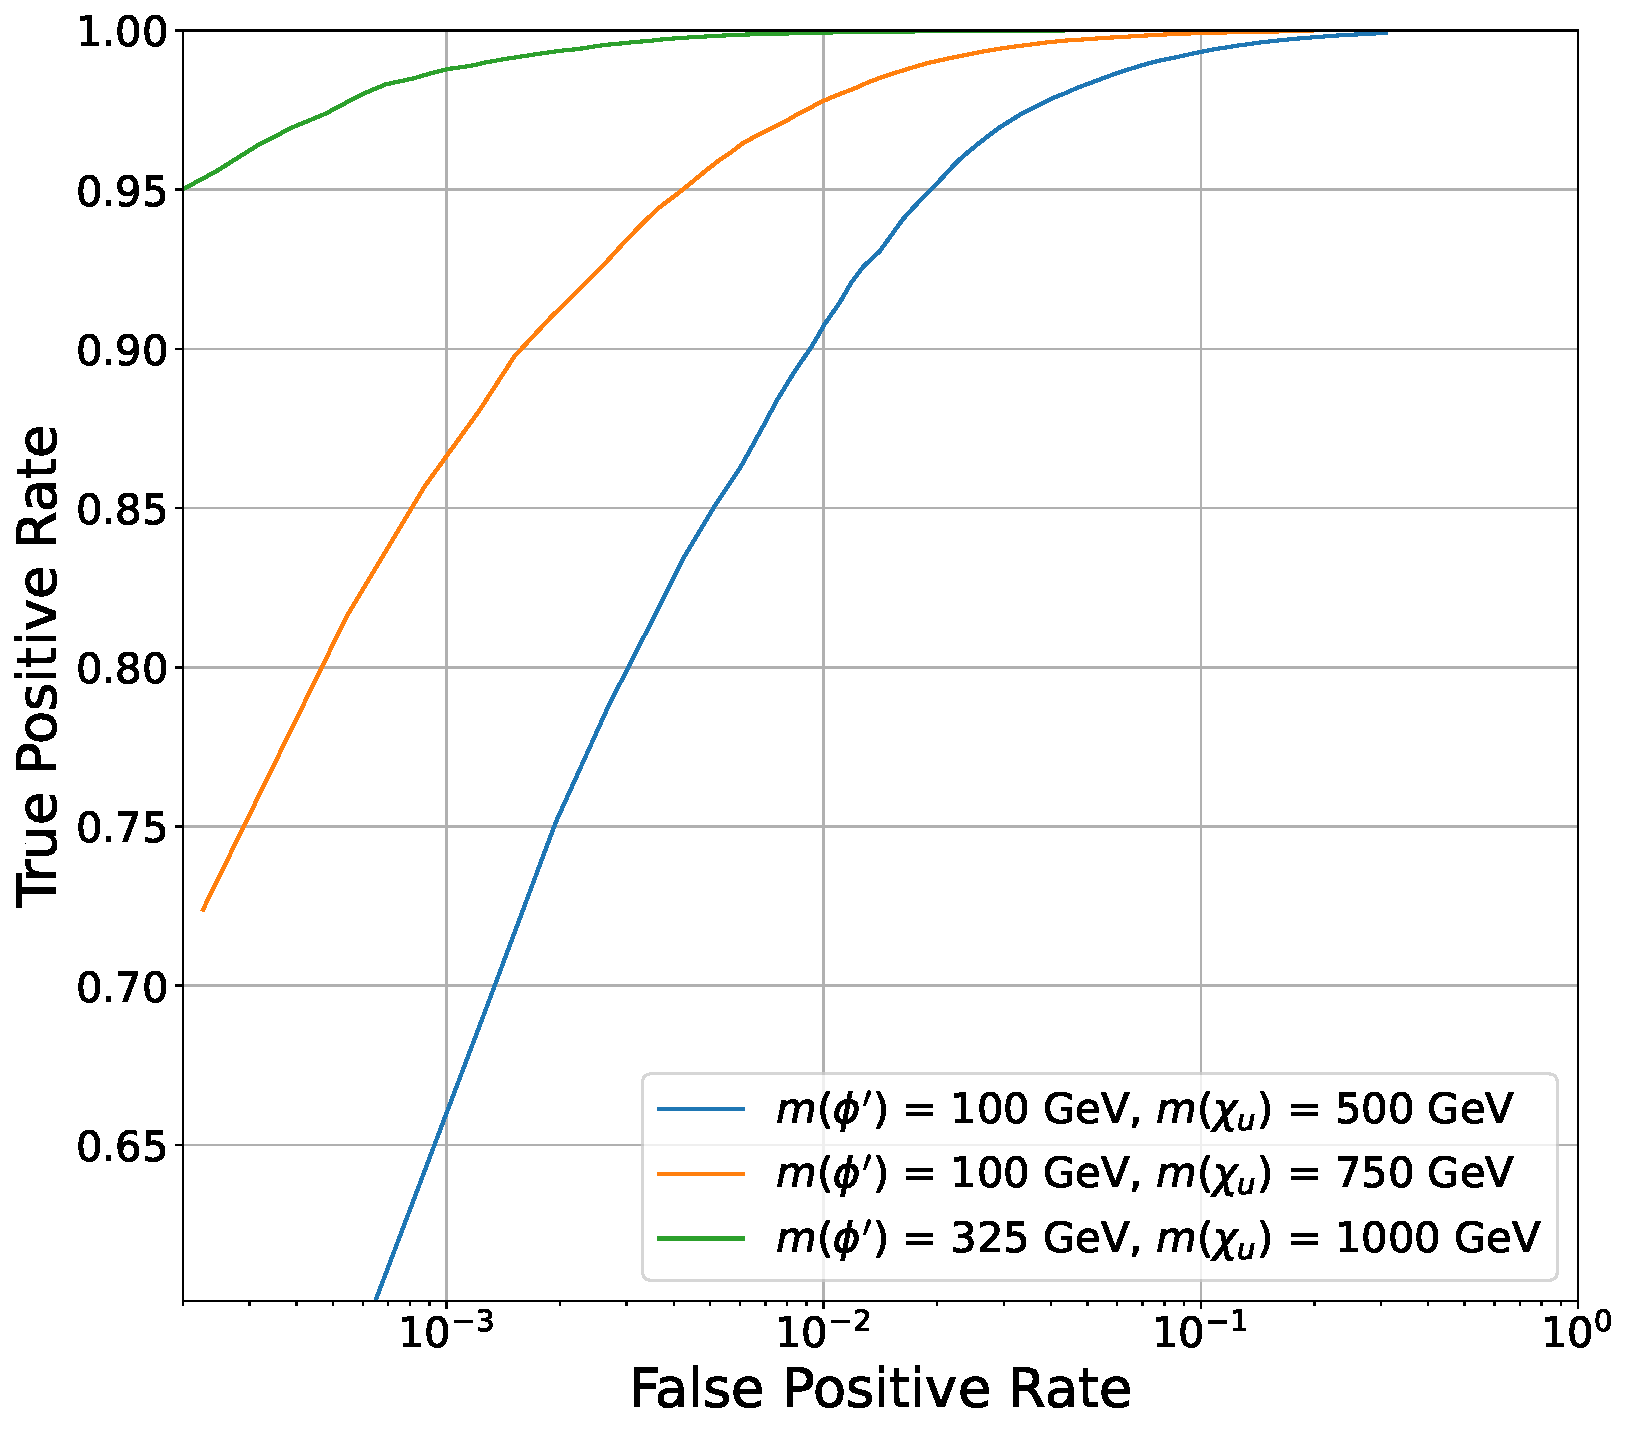
\includegraphics[width=.85\linewidth]{Images/ROC_Curve.pdf}
  \caption{Receiver operating characteristic curve of the BDT algorithm for three different signal benchmark scenarios.}
  \label{fig:ROC}
\end{figure}

\begin{figure}
\centering
  \centering
  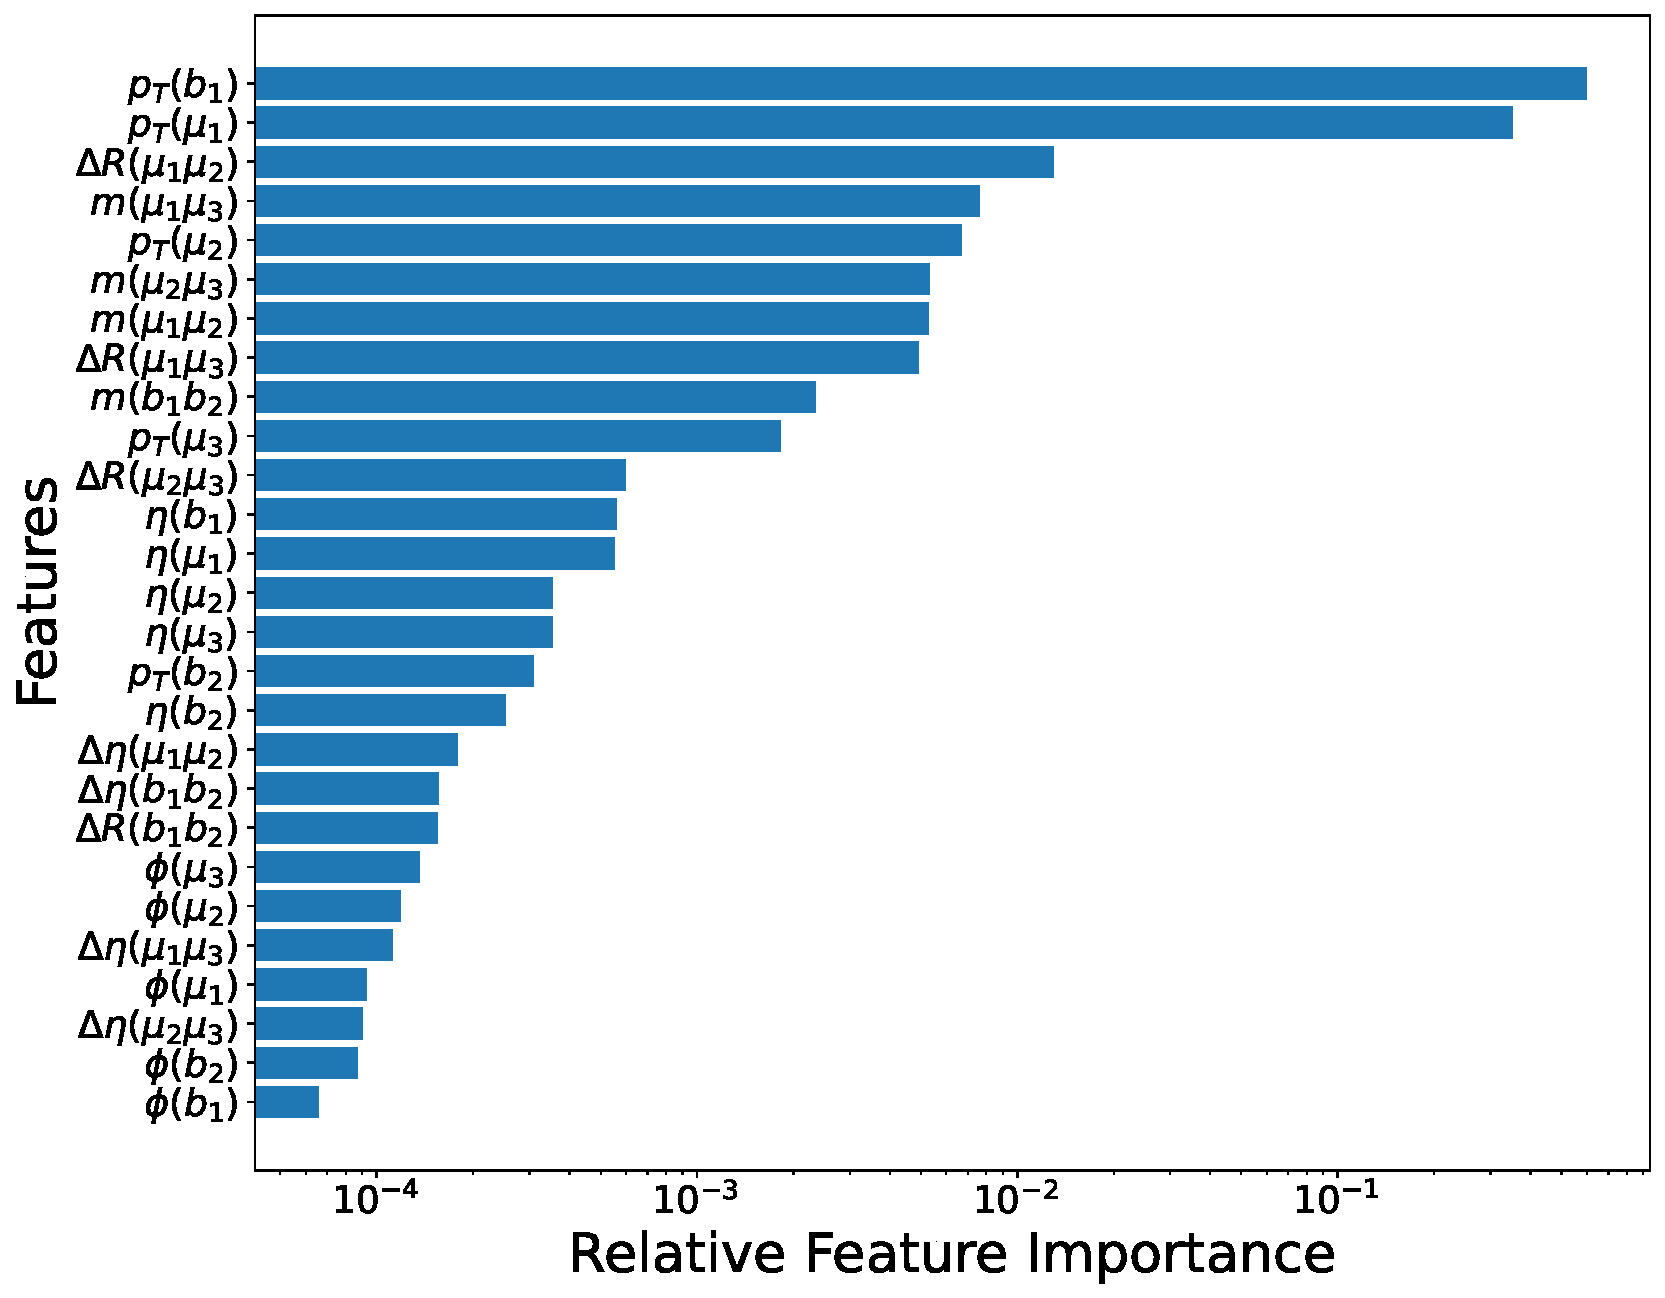
\includegraphics[width=.85\linewidth]{Images/feature_importance.pdf}
  \caption{Relative importance of features in training for a benchmark signal scenario with $m(\phi')=325\, \mathrm{GeV}$ and $m(\chi_\mathrm{u})=2000\, \mathrm{GeV}$.}
  \label{fig:feature_importance}
\end{figure}

The outputs from the BDT machine learning algorithm are used to perform a profile-bin likelihood analysis to estimate the signal significance for a luminosity of 3000 $\mathrm{fb^{-1}}$, corresponding to the expected amount of collected data by the end of the LHC era. For this purpose, the BDT distributions are normalized to cross section times pre-selection efficiency times luminosity for the different signal models. The significance is then calculated using the expected bin-by-bin yields of the BDT output distribution in a profile likelihood fit, using the ROOTFit~\parencite{Butterworth:2015oua} package developed by CERN. The expected signal significance $Z_\text{sig}$ is calculated using the probability of obtaining the same test statistic for the  signal plus background and the signal-null hypotheses, defined as the local $p$-value. Similar to Refs.~\parencite{Florez:2021zoo, Florez:2019tqr, Florez:2018ojp, Florez:2017xhf, VBFZprimePaper, Florez:2016lwi, Leonardi_2020}, the significance  corresponds to the point where the integral of a Gaussian distribution between $Z_\text{sig}$ and $\infty$ results in a value equal to the local $p$-value. The estimation of $Z_\text{sig}$ incorporates  systematic uncertainties. The uncertainty values have been included as nuisance parameters, considering lognormal priors for normalization and Gaussian priors for uncertainties associated with the modeling of the shapes similar to Refs.~\parencite{natalia2021longtermlhcdiscoveryreach, PhysRevD.103.095001}. 

The systematic uncertainties that have been included result from experimental and theoretical constraints.   A 1-5\% systematic uncertainty, depending on the simulated MC sample, has been included to account for the choice of Parton Distribution Function (PDF) set. The systematic uncertainty effect was incorporated following the PDF4LHC~\parencite{Butterworth:2015oua} recommendations. This systematic uncertainty has a small impact on the expected event yields for signal and background, but it does not affect the shape of the BDT output distribution. We additionally considered theoretical uncertainties related to the absence of higher-order contributions to the signal cross sections, which can change the pre-selection efficiencies and the shapes of kinematic variables used as inputs to the BDT algorithm. This uncertainty was calculated by varying the renormalization and factorization scales by $\times 2$, and studying the resulting change in the bin-by-bin yields of the BDT distributions. They are found to be at most 2\% in a given bin. 
%Additional theoretical uncertainties were taken into account, including the potential impact of higher-order contributions to the signal cross sections. These contributions can influence the pre-selection efficiency and shapes of kinematic distributions utilized by the BDT algorithm. The uncertainty associated with this is determined by adjusting the renormalization and factorization scales by a factor of two relative to the nominal value and considering the complete change in the bin-by-bin yields of the BDT output distribution. The maximum impact of these uncertainties in a given bin is found to be 1-3\%. 

Regarding experimental uncertainties, following experimental measurements from CMS on the estimation of the integrated luminosity, a conservative 3\% effect has been included~\parencite{lumiRef}. A 5\% systematic uncertainty associated with the reconstruction and identification of $\mathrm{b}$-quark jets has been included, independent of $p_\mathrm{T}$ and $\eta$ of the $\mathrm{b}$-jet candidates. According to Ref.~\parencite{CMSbtag}, this uncertainty is correlated between signal and background processes with genuine  \textrm{b}-jets and is also correlated across BDT bins for each process. For muons, we include a 2\% uncertainty associated with the reconstruction, identification, and isolation requirements, and a 3\% systematic uncertainty to account for scale and resolution effects on the momentum and energy measurement. 
%For muon reconstruction, identification, and isolation requirements, there is a 1-2\% uncertainty, while a 1-3\% systematic uncertainty is applied to variations in energy/momentum scale and resolution. 
We consider jet energy scale uncertainties ranging from 2-5\%, contingent on $\eta$ and $p_\mathrm{T}$, resulting in shape-based uncertainties on the BDT output distribution. Jet energy scale uncertainties were assumed to range from 1-5\%, contingent on $\eta$ and $p_\mathrm{T}$. These assumptions lead to shape-based uncertainties on the BDT output distribution, varying from 1-2\%. Additionally, we include  a 10\% systematic uncertainty to account for errors in the signal and background predictions. Considering all the various sources of systematic uncertainties, our conservative  estimate yields a total effect of about 20\%. 

\begin{figure}[]
\centering
  \centering
  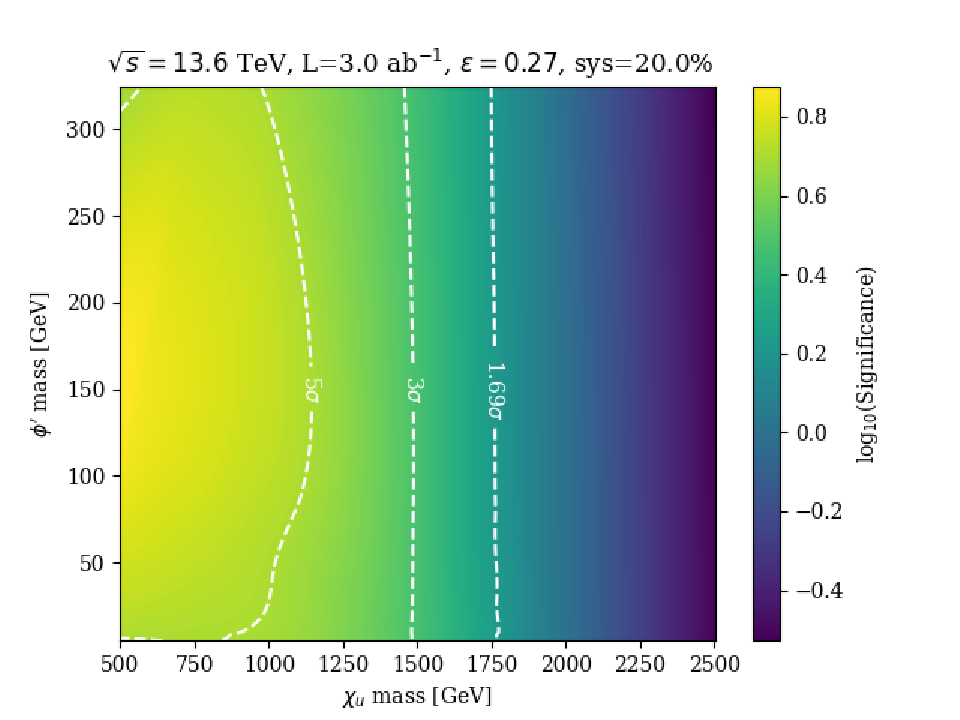
\includegraphics[width=.95\linewidth]{Images/significance.pdf}
  \caption{Signal significance for the high luminosity LHC era, considering with 3000  $\mathrm{fb}^{-1}$ of collected data.}
  \label{fig:/significance_3000}
\end{figure}

Figure~\ref{fig:/significance_3000} shows the expected signal significance considering an integrated luminosity of 3000 $\mathrm{fb^{-1}}$. The significance is shown as a heat map in a two-dimensional plane for different $\phi'$ and $\chi_{\mathrm{u}}$ masses. The x-axis corresponds to $m(\chi_\mathrm{u})$, the y-axis to $m(\phi')$, and the heat map to log$_{10}(\mathrm{Z}_{sig})$. The white dashed lines are contours of constant signal significances of $1.69 \sigma$,  $3\sigma$ and  $5\sigma$ to represent regions of possible exclusion, evidence of new physics, and discovery, respectively. Under these conditions, $\phi'$ ($\chi_{\mathrm{u}}$) masses ranging from 1 to 325 \textrm{GeV} (500 to 1800 \textrm{GeV}) can be probed. The range for a discovery with $5\sigma$ signal significance varies from $\chi_{\mathrm{u}}$ masses from $m(\chi_{\mathrm{u}}) = 770$-1100 \textrm{GeV}, depending  $m(\phi^{'})$. For large $m(\chi_\mathrm{u})$, the significance is almost independent of $m(\phi')$ because the primary discriminating feature—the boosted $b$-quark originating from $\phi'$—is driven predominantly by the large $m(\chi_\mathrm{u})$, with the kinematic impact of $m(\phi')$ being relatively negligible.


